\section{Themes in the IMCL Group}

The research of the IMCL group is mainly focused on 4 Themes : Smart sensing, wireless networks, mobile cloud computing, big data, and pervasive computing. Under these themes, we have a total of 19 research topics. The research themes and the corresponding research topics are shown in Fig. 1.

\begin{figure*}
\begin{center}
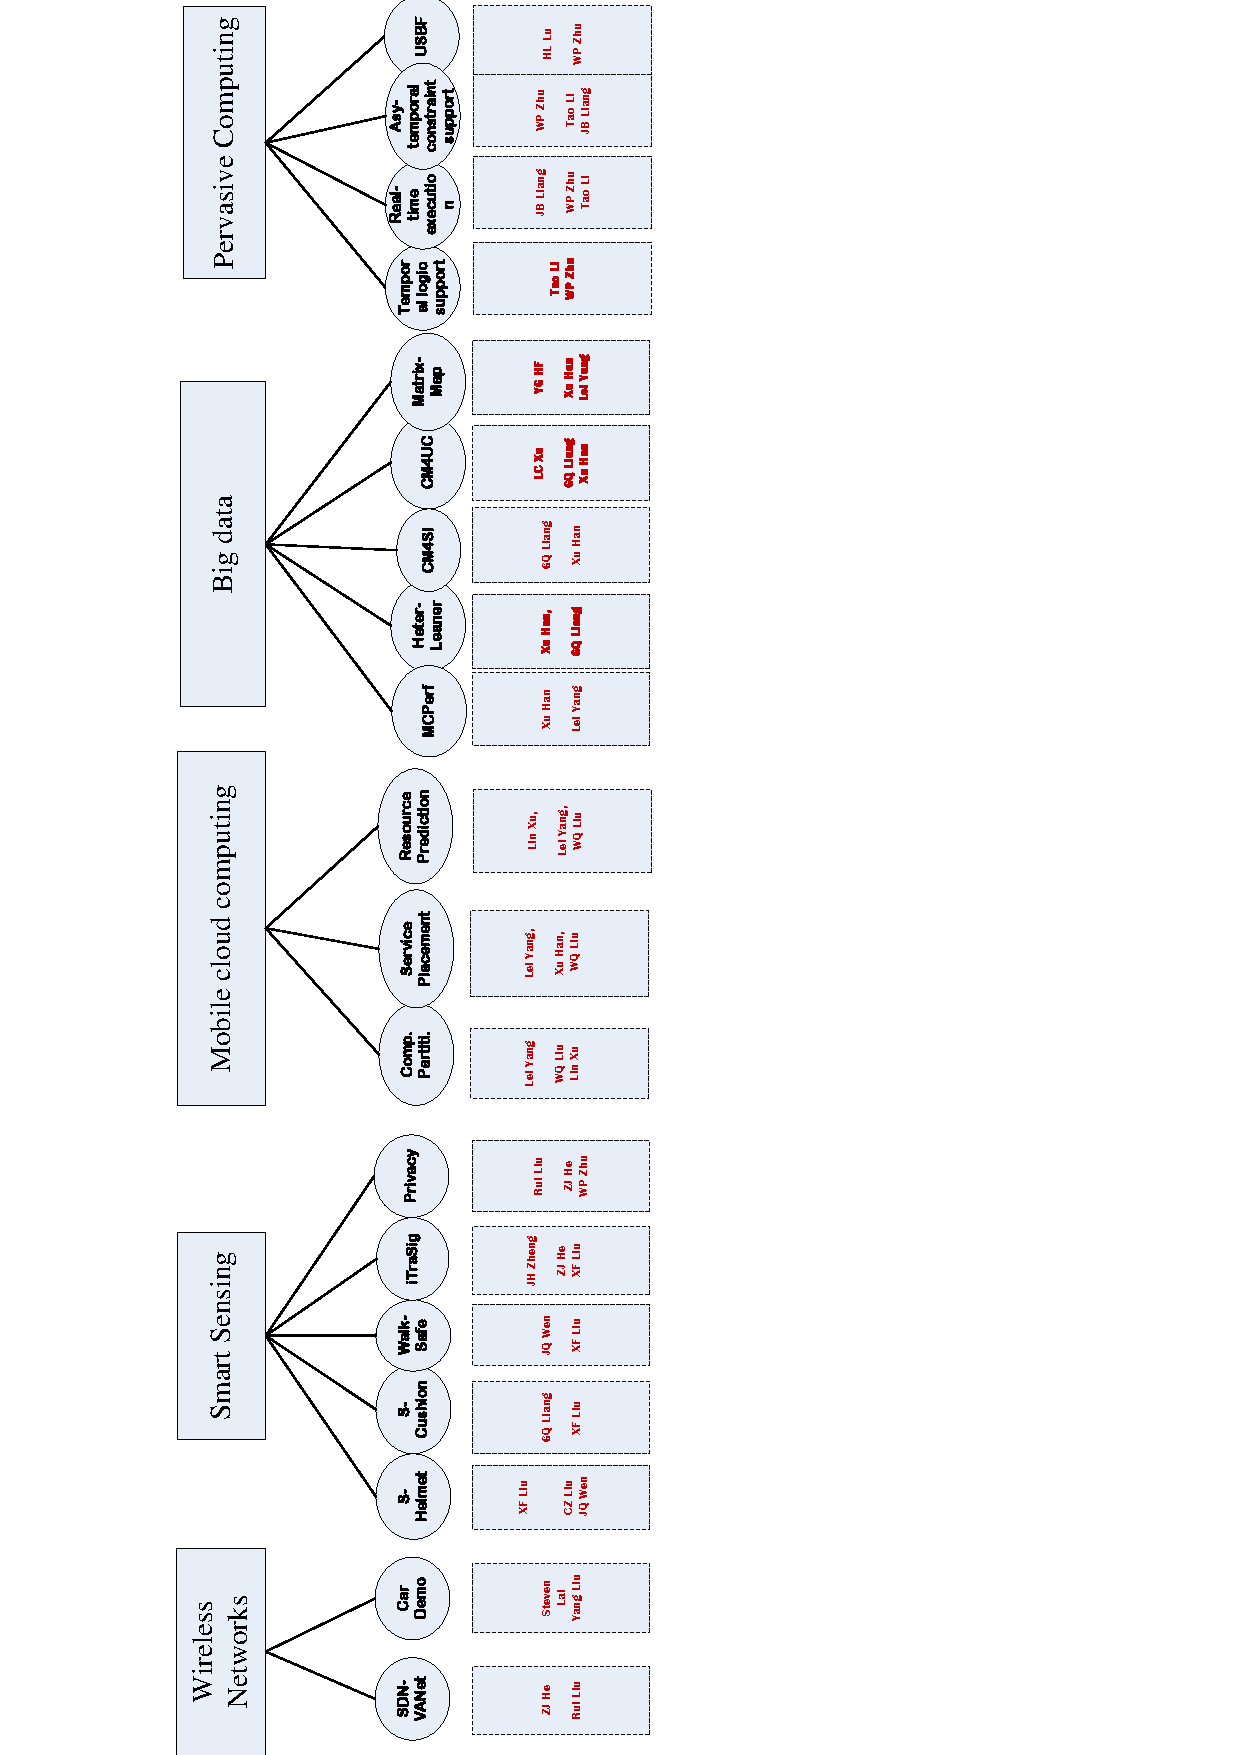
\includegraphics[angle=0,width=8cm,height=24cm]{Structure2.pdf}

\end{center}
\caption{} %The time intervals of received packets. .}
\label{fig:topics}
\end{figure*}


\textbf{1. Wireless Networks}

A heterogeneous wireless networking technology for seamless communication and mobility
Smart phones have taken the world by storm, with their global sales set to hit 1 billion by 2010.  On top of normal phone functions, a smart phone serves in an additional capacity as a mobile computing device. This marks a rapid shift in web surfing habits from the desktop to the mobile phone. In a parallel move, consumers want to access the Internet anytime, anywhere.  To make the Internet more mobile, we have developed a platform of heterogeneous advanced wireless networks known as ��HAWK��, which delivers an unprecedented level of mobility and coverage for Internet access that the mobile generation would love.

With this revolutionary technology in place, mobile users would roam smoothly and continuously as they hop across Wi-Fi, 2.5G and 3G cellular networks.  The transition is totally seamless and transparent, thanks to HAWK��s seamless handoff technology which dramatically speeds up the handoff process, allows the switching to occur automatically and makes intelligent decisions to adjust the quality of multimedia service to network capacity. As a result, users no longer lose connections and do not need to manually reconnect again while they are on the move, making their Internet access much smoother and more convenient, especially during Internet phone call or video conferencing.  While moving through the metropolitan cities, people can now enjoy their on-line games and the upcoming 2010 World Cup live broadcast seamlessly and continuously.

Furthermore, the HAWK uses advanced Wi-Fi meshes to link up hotspots, trying to extend Wi-Fi coverage beyond islands of broadband by filling the void in between.  Better still, it enables Wi-Fi access to penetrate even the most impossible locations, such as rough terrain or places with no fixed infrastructure.  Given its excellent reliability, this unique technology delivers unprecedented coverage of Wi-Fi for unbeatable online experience.  In the future, mobile users can enjoy at all times high quality, high speed, and unlimited broadband access wherever they go, at a higher rate than 3G.

In addition, we also focus on vehicular networks. We have developed vehicular networks based on software-defined network (SDN).


\textbf{2. Smart Sensing}

The objective of this theme is to realize efficient sensing, computing and communication in resource-constraint wireless and mobile networks for a wide range of applications such as wireless sensor network based structural health monitoring, human centric healthcare based on smart sensors, smartphone applications, localization systems, etc.

Figure \ref{fig:WNWSN} shows a research framework that covers the main topics we are interested. Please refer to the research topics under this theme for details.%The research topics are mainly focused on distributed computing in data-intensive and computation-complex applications; crowd souring,

\begin{figure}
	\centering
		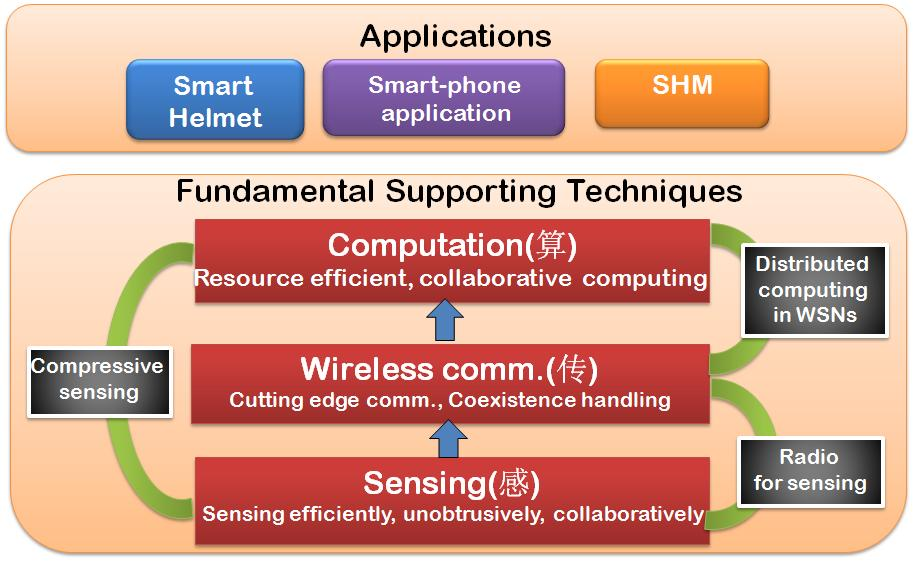
\includegraphics[width=0.6\textwidth,height=.4\textwidth]{WNWSN.jpg}
	\caption{Research Framework of wireless networks and wireless sensor networks group}%The time intervals of received packets. .}
	\label{fig:WNWSN}
\end{figure}

\textbf{3. Mobile cloud computing}

The objective of this them is to design compute-intensive or data-intensive mobile applications by using cloud computing technology. is not trivial to develop compute-intensive applications on mobile devices with the aim of achieving low latency and energy consumption. It is also challenging to develop data intensive mobile applications, since it re-quires effective ways to process and analyze the big data from the mobile applications. To solve these two challenges, we have dedicated many efforts in developing algorithms and mechanisms at different technical layers such as resource management, data management, computation scheduling and programming abstraction.

Figure \ref{fig:MCC} shows a research framework that covers the main topics in the field of mobile cloud computing. The topics are classified into various system layers: resource management, computation and data management, programmng models and applications. Note that the resources in mobile cloud environment consist of the networking, computation and storages from mobile nodes, cloudlets distributed at the network edge and centralized data centers on the Internet. At resource management layer, the main goal is to abstract the resources from various distributed hosts, and provision them as services to consumers. The research issues at this layer may be quite different depending on specific system models and objectives. For example, in ad hoc based mobile cloud model, one issue is to design effective mechanism to incentive more peers to participate into the system and share their computing resources.


\begin{figure}
	\centering
		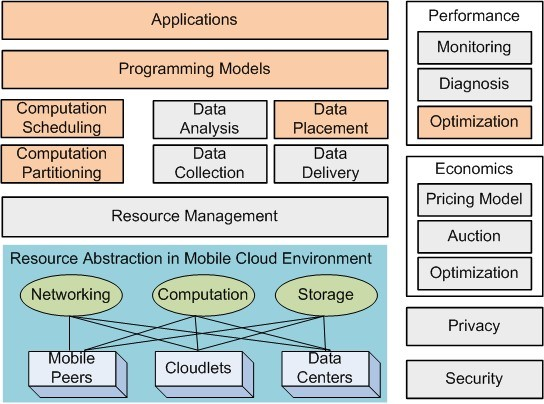
\includegraphics[width=0.6\textwidth,height=.4\textwidth]{MCCFramework.jpg}
	\caption{Research framework of mobile cloud computing} %The time intervals of received packets. .}
	\label{fig:MCC}
\end{figure}

On the topic of resource management layer, we are facing a few issues related to computation and data management. One hot topic studied extensively recently is computation partitioning, i.e., to decide for mobile devices which parts of application should be computed on the mobile devices and which parts should be offloaded onto cloud, such that certain objective like computation time and energy consumption is optimized. Highly associated with computation partitioning, another issue is computation scheduling of the off-loadings from mobile users onto the data center resources.

Besides computation related research, there exist continuous efforts on the data centric research in mobile cloud, which is named as data management in our framework. The re-search area assumes a smart mobile cloud system that is able to collect, analyze, store (place), and deliver the data intelligently and efficiently. To be specific, data collection focuses on how to aggregate/fuse and then gather the data from multiple mobile devices to the centralized cloud in an energy efficient way. Data analysis particularly focuses on the design of computing platforms for data processing, and algorithms for data analysis. Data placement and data delivery aims to provide good quality data services for the end users.

At programm model layer, much research efforts have been dedicated on the design of easy-to-use programming models for develop various mobile cloud applications. Due to the inherent data intensive property of most mobile cloud applications, one research issue lies on how to design easy-to-use programming models and interfaces for big data application developers. At application layer, researchers are focusing on development of novel applications re-lying on mobile cloud system technologies. Some popular applications that inherently need to leverage the cloud computing are mobile interactive perception application, mobile augmented reality, community sensing applications and so on.

The right side of the framework lists four interests that could be focused by researchers: performance, economics, privacy and security. The four interests are classified from the perspective of research objectives, and involve the techniques across all the layers. The performance related topics include the performance monitoring, diagnosis and optimization. The economics cover the topics of pricing models and auction models, and monetary cost optimization.

Our research focuses on a few but not all topics in the framework. First, we have dedicated most efforts on the performance optimization specifically at the layer of computation and data management. Specifically we focus on the issue of computation partitioning and scheduling, and data placement. Second, we also have done some works on programming models for big data process. We focus on developing a framework for integrating existing big data programming models using a unified interface. Third, we have been developing mobile multimedia applications by mobile cloud technologies. One novel application we focus on is touch free HCI on smart phones. We have designed live video based gesture recognition algorithms, and aim to optimize the performance on smart phones.



\textbf{3. Big Data}

The objective of this theme is to provide methods and mechanisms for collecting, organizing, processing and analyzing huge volumes of data. With the capability of analyzing big data, we can uncover hidden patterns, unknown correlations and other useful information to make better decisions. It is challenging to design models and algorithms for parallel data processing and data mining in various application areas. Meanwhile, since we need to utilize cloud resources effectively in processing and analyzing big data, it is important to ensure the performance of data-intensive applications in cloud environment. In face of these challenges, we make many efforts in designing algorithms and mechanisms at different technical layers such as data analysis, data processing, data management, etc.

As shown in Fig. \ref{fig:BD}, our research framework covers the main topics in the field of big data analytics. The topics are classified into various system layers. These layers differ in function, system level, specific interface, and the extent of interaction with users. In the hierarchical structure of this framework, three primary layers are defined for decision-making processes, including data processing, data analysis and application layers.

\begin{figure}
	\centering		 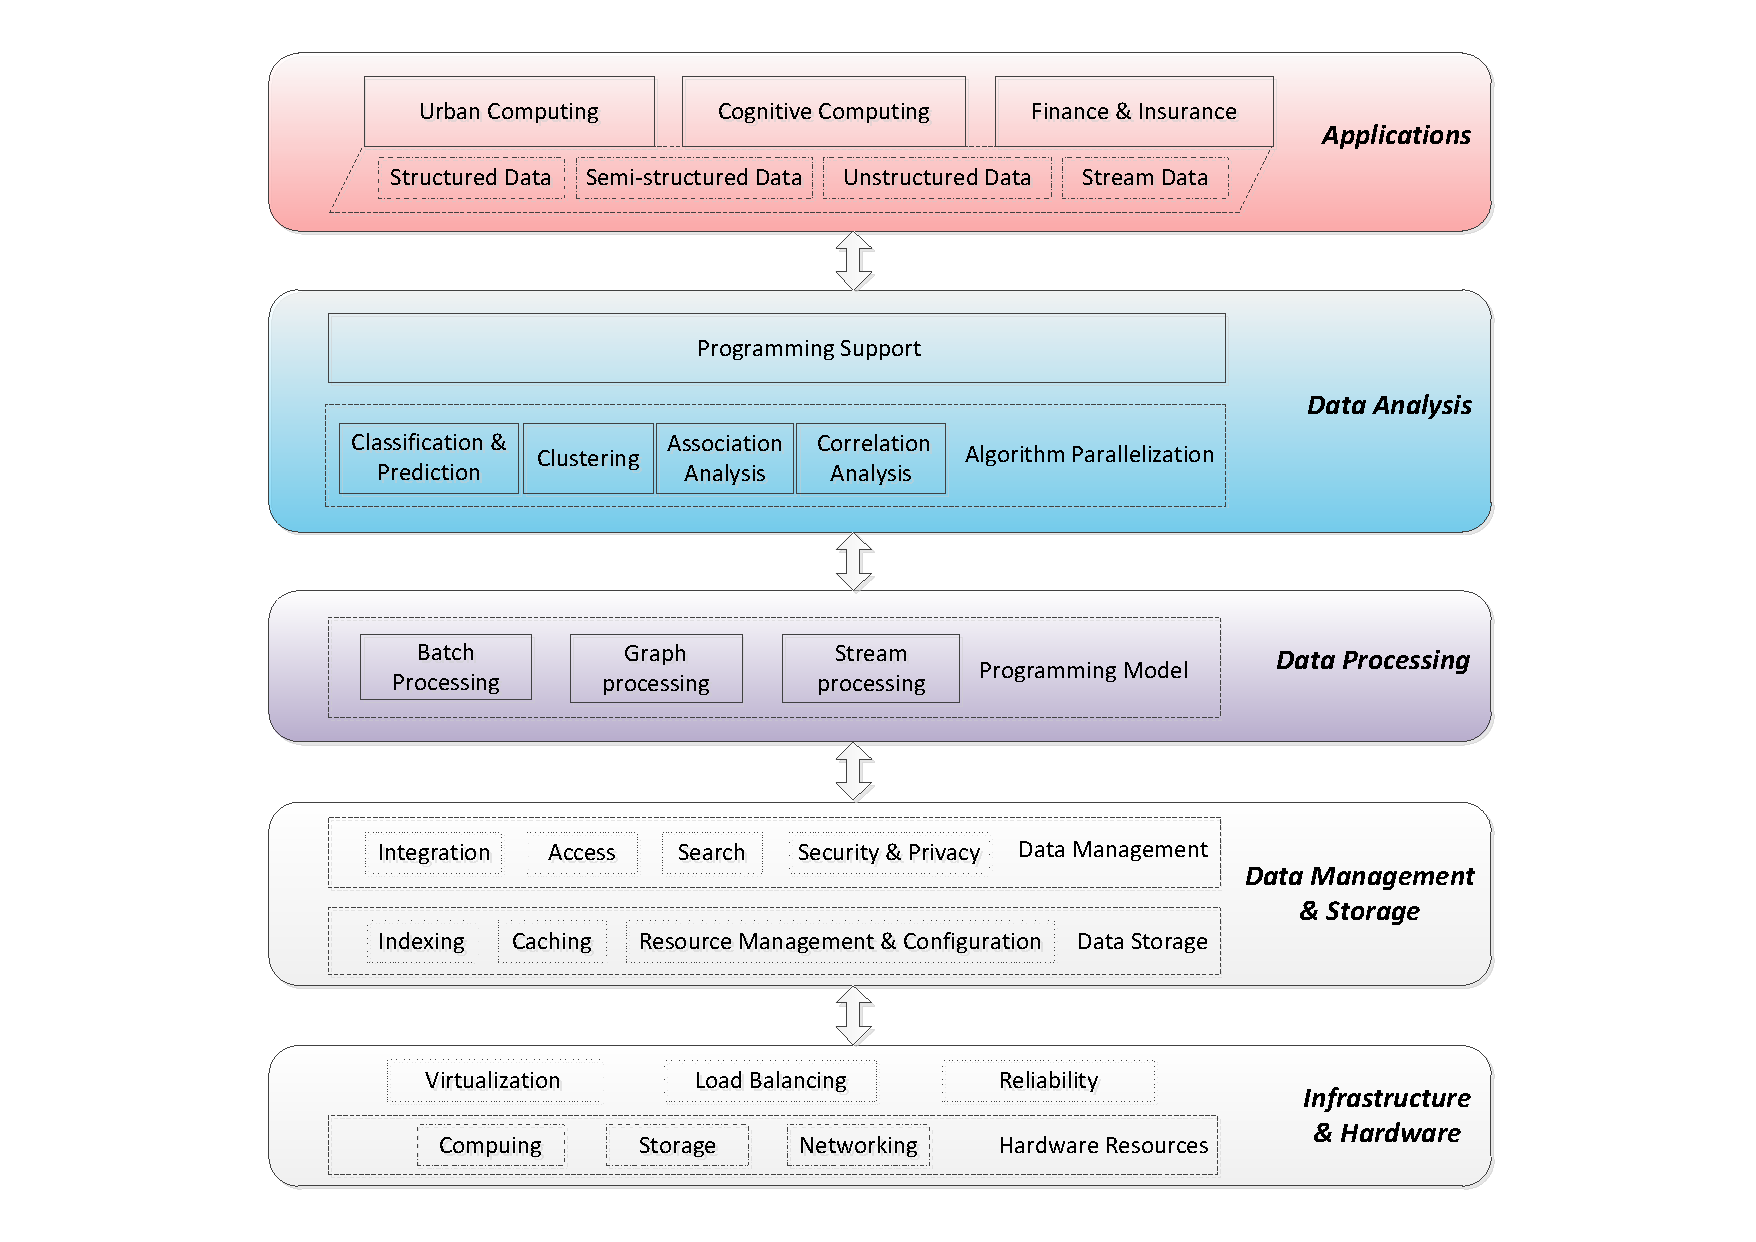
\includegraphics[height=.6\textwidth]{BD.pdf}
	\caption{Research Framework of Big Data Group}%The time intervals of received packets. .}
	\label{fig:BD}
\end{figure}




\textbf{4. Pervasive Computing}

The objective of this theme is to develop theories/methodologies for building high performance pervasive computing systems, and ease its development/testing by providing various tools. Among pervasive computing, we currently focus on two important applications, distributed MEMS (micro-electro-mechanical systems), and searching and browsing cyber-physical objects. For the former one, we aim to provide programming support and design efficient and effective algorithms for distributed MEMS. And for the latter one, we aim to develop efficient approaches for the browsing and searching the objects in cyber-physical systems. We believe that our research will make valuable contributions to the pervasive computing and the internet of things, and make people's life easier, healthier, and happier.

Figure~\ref{fig:MEMS} shows a research framework of programming distributed MEMS. There are three aspects for programming distributed MEMS, named programming principle, programming paradigm, and supported features. The programming principle defined the view of programmers to the MEMS, either ensemble-based or individual node-based. The latter follows the traditional distributed development, considering the distribution of data and function in individual nodes and communication among them. On the contrast, the ensemble-based way considers all the individual nodes as a whole and specifies the common rules for them to achieve objectives. All the underlying data distribution and communication are left to the system implementation.  For the programming paradigm, the application development can be based on declarative languages or imperative languages. Finally, the sup-ported features include scalability, fault-tolerance, real-time, feedback control, etc. Real-time support is our current focus, and can be investigated on the topics on the time specification, time estimation, scheduling, and real-time control

\begin{figure}
	\centering		 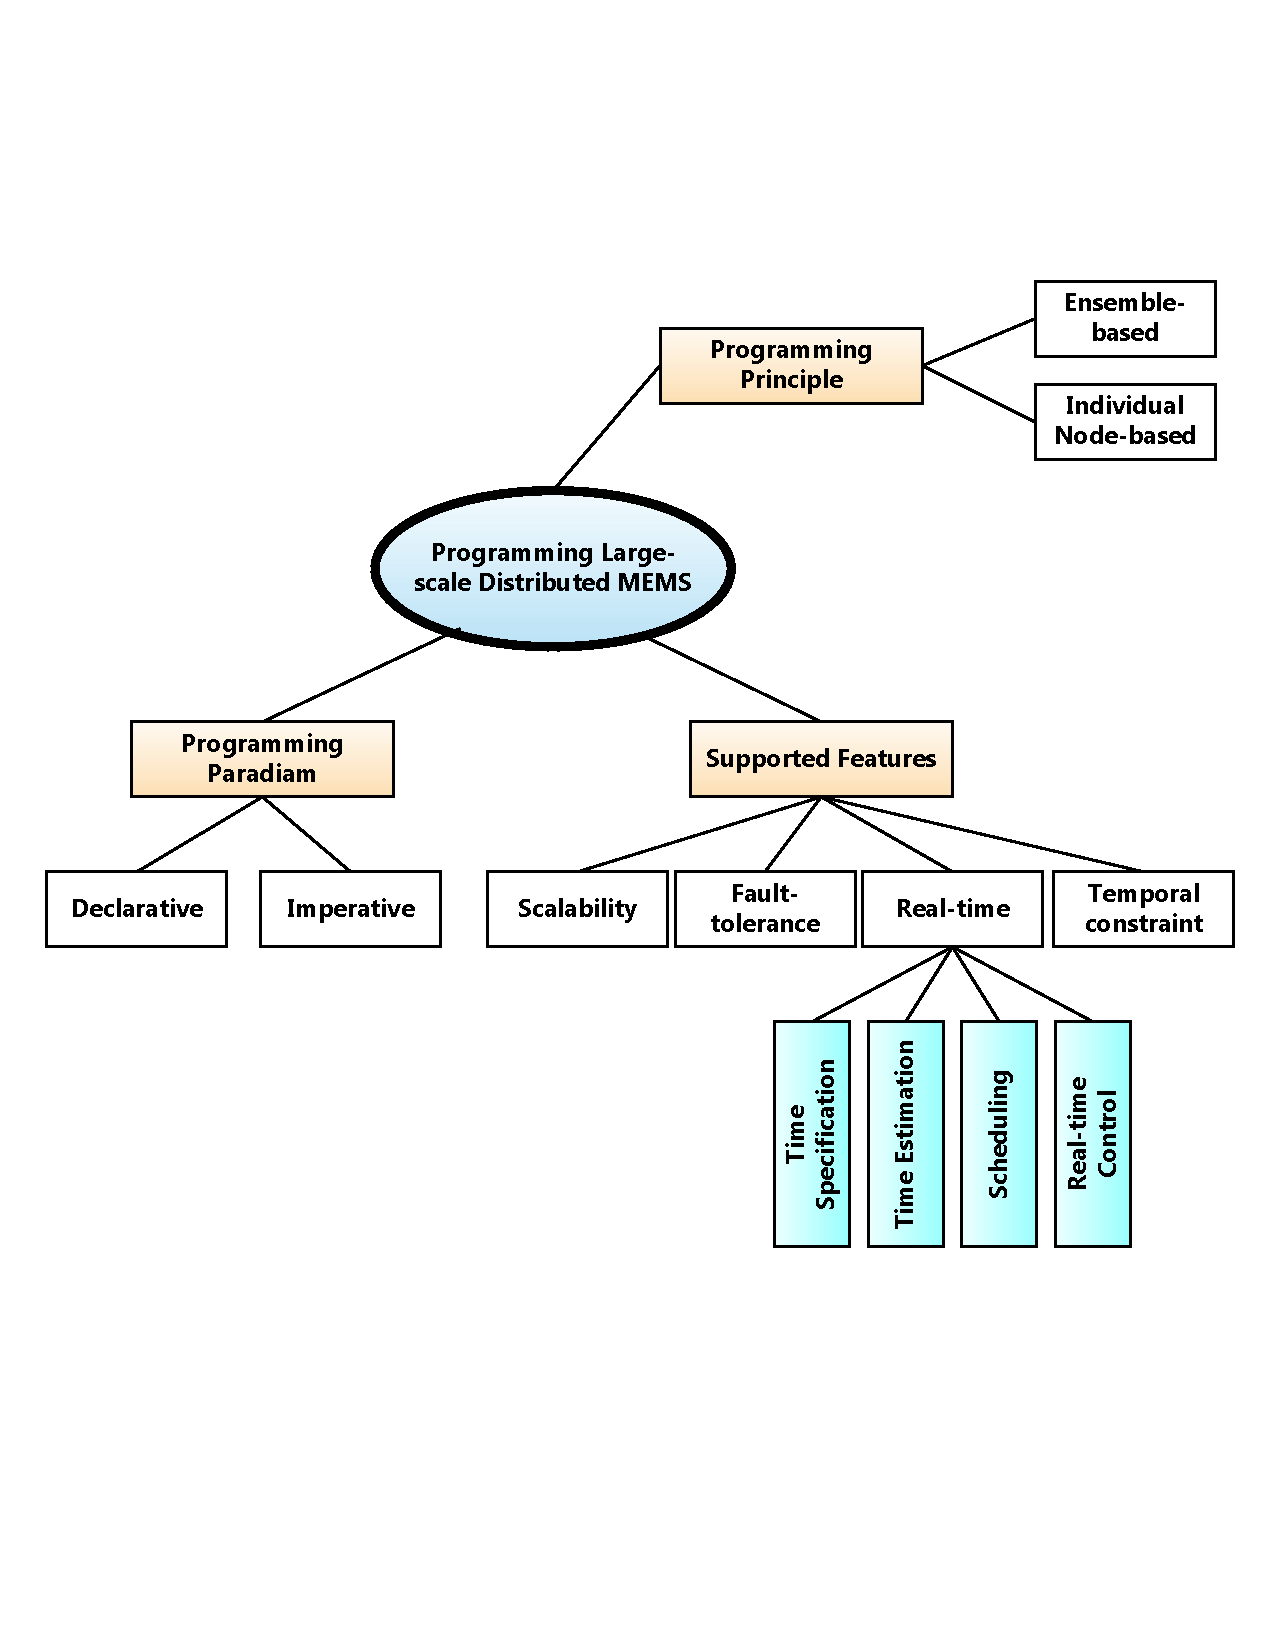
\includegraphics[height=.6\textwidth]{MEMS.pdf}
	\caption{Research Framework of Programming Support for Distributed MEMS}%The time intervals of received packets. .}
	\label{fig:MEMS}
\end{figure}

Figure \ref{fig:USBF} shows a research framework that covers the main topics of searching and browsing cyber-physical objects.
The topics are classified into five layers: information collection, communication and networking, modeling, programming support, and application. Information collection layer is responsible for collecting information from objects in the cyber world and in the physical world. It needs to conduct identification, localization, spatio/temporal correlation, and social correlation to different objects. Communication and network layer is responsible for connect different objects into a network for the ease of searching and browsing. The major functions include access, rout-ing, caching, service handoff, etc. On the top of it, proper modeling approaches are needed for the operation and development in such systems. The modeling need to cover the objects, its at-tributes, relationship among objects, services, and behaviors. Based on this model,  some key programming supports are provided,  including storage management, index building, query matching, result ranking, relation detection and inference, to the user for the ease of the application development, object searching and object browsing.

\begin{figure}
	\centering		 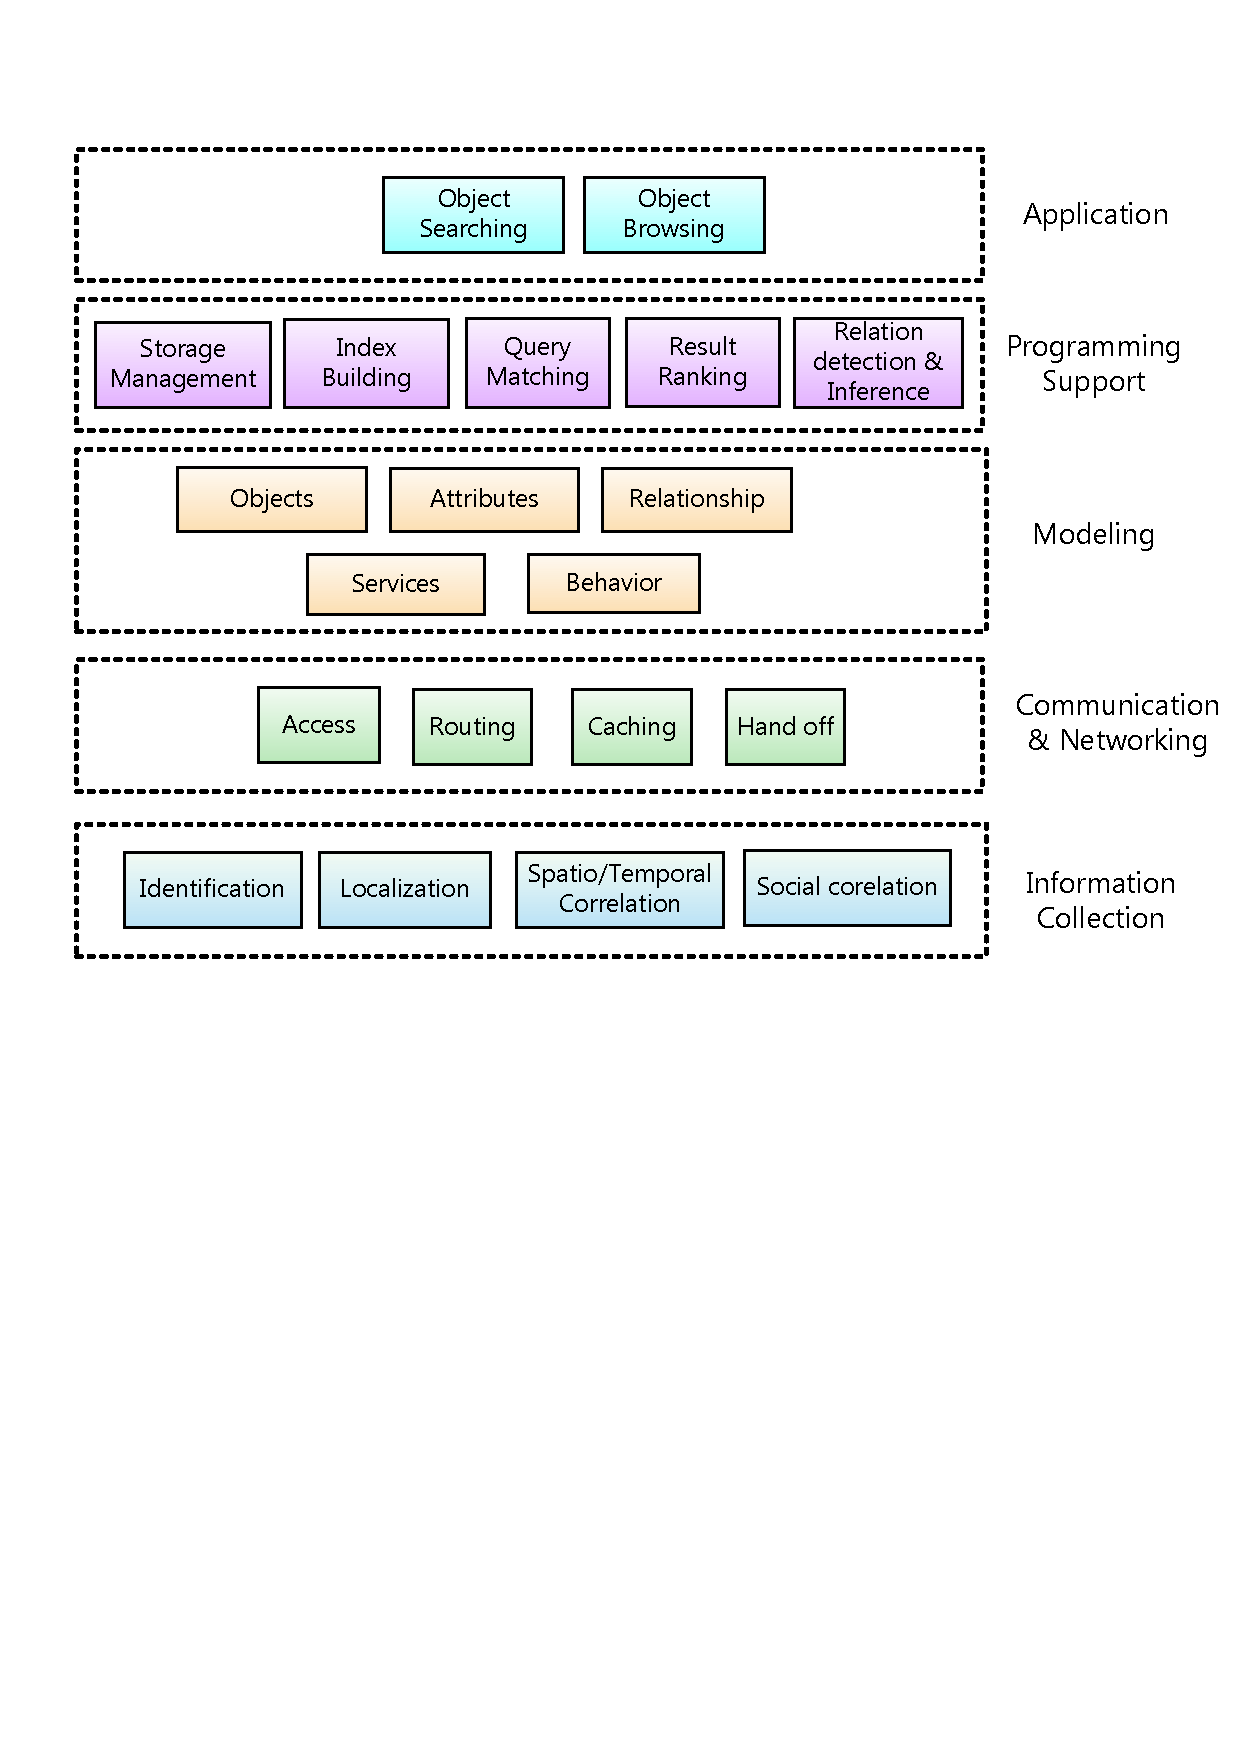
\includegraphics[height=.6\textwidth]{USBF.pdf}
	\caption{Research Framework of Searching and Browsing Cyber-physical Objects}%The time intervals of received packets. .}
	\label{fig:USBF}
\end{figure}
